\documentclass{beamer}\usepackage[]{graphicx}\usepackage[]{color}
%% maxwidth is the original width if it is less than linewidth
%% otherwise use linewidth (to make sure the graphics do not exceed the margin)
\makeatletter
\def\maxwidth{ %
  \ifdim\Gin@nat@width>\linewidth
    \linewidth
  \else
    \Gin@nat@width
  \fi
}
\makeatother

\definecolor{fgcolor}{rgb}{0.345, 0.345, 0.345}
\newcommand{\hlnum}[1]{\textcolor[rgb]{0.686,0.059,0.569}{#1}}%
\newcommand{\hlstr}[1]{\textcolor[rgb]{0.192,0.494,0.8}{#1}}%
\newcommand{\hlcom}[1]{\textcolor[rgb]{0.678,0.584,0.686}{\textit{#1}}}%
\newcommand{\hlopt}[1]{\textcolor[rgb]{0,0,0}{#1}}%
\newcommand{\hlstd}[1]{\textcolor[rgb]{0.345,0.345,0.345}{#1}}%
\newcommand{\hlkwa}[1]{\textcolor[rgb]{0.161,0.373,0.58}{\textbf{#1}}}%
\newcommand{\hlkwb}[1]{\textcolor[rgb]{0.69,0.353,0.396}{#1}}%
\newcommand{\hlkwc}[1]{\textcolor[rgb]{0.333,0.667,0.333}{#1}}%
\newcommand{\hlkwd}[1]{\textcolor[rgb]{0.737,0.353,0.396}{\textbf{#1}}}%
\let\hlipl\hlkwb

\usepackage{framed}
\makeatletter
\newenvironment{kframe}{%
 \def\at@end@of@kframe{}%
 \ifinner\ifhmode%
  \def\at@end@of@kframe{\end{minipage}}%
  \begin{minipage}{\columnwidth}%
 \fi\fi%
 \def\FrameCommand##1{\hskip\@totalleftmargin \hskip-\fboxsep
 \colorbox{shadecolor}{##1}\hskip-\fboxsep
     % There is no \\@totalrightmargin, so:
     \hskip-\linewidth \hskip-\@totalleftmargin \hskip\columnwidth}%
 \MakeFramed {\advance\hsize-\width
   \@totalleftmargin\z@ \linewidth\hsize
   \@setminipage}}%
 {\par\unskip\endMakeFramed%
 \at@end@of@kframe}
\makeatother

\definecolor{shadecolor}{rgb}{.97, .97, .97}
\definecolor{messagecolor}{rgb}{0, 0, 0}
\definecolor{warningcolor}{rgb}{1, 0, 1}
\definecolor{errorcolor}{rgb}{1, 0, 0}
\newenvironment{knitrout}{}{} % an empty environment to be redefined in TeX

\usepackage{alltt}


% If you have a file called "university-logo-filename.xxx", where xxx
% is a graphic format that can be processed by latex or pdflatex,
% resp., then you can add a logo as follows:
\title{How often does the best team win? A unified approach
to understanding randomness in North American sport}
% \subtitle
% {for Graduate Students} % (optional)
 

%\author[Ofer Harel] % (optional, use only with lots of authors)
%{Ofer Harel\inst{1} and  Gregory Matthews\inst{2}}

\author{Gregory Matthews $^{1}$, Ben Baumer $^{2}$, and Mike Lopez $^{3}$ }



%  \inst{1}
  %Department of Statistics\\
  %University of Connecticut

% - Use the \inst{?} command only if the authors have different
%   affiliation.
\institute [Loyola] % (optional, but mostly needed)
{
  $^{1}$Loyola University Chicago\\
  
  
  $^{2}$Smith College\\
  
  
  $^{3}$Skidmore College\\
  
}



% - Use the \inst command only if there are several affiliations.
% - Keep it simple, no one is interested in your street address.

\date[October 2016] % (optional)
{October, 2016} %Date / Occasion}
\IfFileExists{upquote.sty}{\usepackage{upquote}}{}
\begin{document}
%\SweaveOpts{concordance=TRUE}

\begin{frame}
  \titlepage
\end{frame}

\begin{frame}
  \frametitle{Outline}
  \tableofcontents
  % You might wish to add the option
  % [pausesections]
\end{frame}


\section{Introduction}
%Opening R - some basics (getwd setwd)
%Data Management

%\begin{frame}{}
%\begin{itemize}
%\item Basically everyone who is interested in sports is interested in the question ``Is team $i$ better than team $j$?  
%\item How do we measure team strength within a league?
%\item If we knew the relative team strengths we could view the outcome as a draw from a random variable with some win probability for team $i$. 
%\end{itemize}
%\end{frame}

\begin{frame}{Main Goal}
\begin{itemize}
\item Our main goal with this research is to compare all four of the major North American sports (Football (NFL), Basketball (NBA), Baseball (MLB), and Hockey (NHL)) on the same scale.  
\end{itemize}
\end{frame}

\begin{frame}{Common question in sports}
\begin{itemize}
\item Contrasting league-level characsteristics in economics (Leeds and Von Allmen, 2004)
\item Estimating game-level probabilities in statistics (Glickman and Stern, 1998)
\item Classifying future game winners in forecasting (Boulier and Stekler, 2003)
\end{itemize}
\end{frame}

\begin{frame}{Competitive Balance}
\begin{itemize}
\item Noll, 1988, Scully, 1989, and Gini Coefficient (Mizak et al. 2005)
\item Use win percentage as a proxy for team strength.  
\item However, these methods have some undersirable properties.  
\item For instance, Noll-Scully increases, on average, with the number of games played, so it's hard to compare across league with different number of games (e.g. NFL vs MLB)
\end{itemize}
\end{frame}

\begin{frame}{Our approach}
\begin{itemize}
\item A simple ways of estimating team strength in leagues is the Bradley-Terry Model (Bradley and Terry, 1952) 
\item Application to football (Glickman and Stern (1998), Glickman and Stern (2017))
\item We use a modified version of the model proposed in Glickman and Stern (1998)
\item Instead of estimating win probabilities we work backwards.  
\item We assume that betting markets offer unbiased and low-variance estimates of true probabilities.  
\item Betting markets are efficient (Harville, 1980; Stern, 1991; Carlin, 1996; Colquitt et al. 2001; Nichols ,2012; Paul and Wienback, 2014; Spann and Skiera, 2009; Gander et al., 1988; Lacey, 1990)
\end{itemize}
\end{frame}


%This manuscript aims to fill these voids. Instead of estimating team strengths within a single sport and using those estimates to generate estimated win probabilities, we work backwards. First, we suppose---and work to validate---that betting market probabilities provide unbiased and low-variance estimates of the true probabilities of wins and losses in each game. Second, using the logit transform of those probabilities, we propose a modified Bayesian state-space model that captures implied team strength and variability. An advantage of this model is that it can be applied uniformly across leagues. Finally, by looking at posterior estimates of within and between season variability, as well as the overall dispersion in team strength estimates, we present unique league-level contrasts which, to this point, have been difficult to capture. As examples, we find that season-to-season reversion to the average is highest in the NHL, and that the gaps in talent in the NBA and NFL overwhelm those of the NHL and MLB.  Additionally, we quantify the relative home advantage for each franchise, as well as between-league differences in the randomness in postseason play. All together, our results better inform an understanding of the dispersion of both talent and randomness in sport. 

\section{Data}
\begin{frame}[fragile]{What data do we have}
\tiny
% latex table generated in R 3.3.1 by xtable 1.8-2 package
% Fri Oct 14 18:41:39 2016
\begin{table}[ht]
\centering
\begin{tabular}{lrrrrrrr}
  \hline
sport & games & num\_teams & home\_wp & N\_bets & mean\_home\_p & N\_results & coverage \\ 
  \hline
mlb & 21854 &   30 & 0.542 & 21854 & 0.549 & 24299.000 & 0.899 \\ 
  nba & 10781 &   30 & 0.598 & 10781 & 0.619 & 12059.000 & 0.894 \\ 
  nfl & 2294 &   32 & 0.567 & 2294 & 0.590 & 2560.000 & 0.896 \\ 
  nhl & 10535 &   30 & 0.551 & 10535 & 0.566 & 10564.000 & 0.997 \\ 
   \hline
\end{tabular}
\caption{Summary of cross-sport data. Note that we have near total coverage (betting odds for every game) across all four major sports during the 2005--2014 regular seasons.} 
\label{tab:bigfour}
\end{table}


\end{frame}

%Each dot represents a bin of implied probabilities rounded to the nearst hundredth. The size of each dot is proportional to the number of games that lie in that bin. We note that across all four major sports, the observed winning percentages accord with those implied by the betting markets. The dotted diagonal line indicates a completely fair market where probabilities from the betting markets correspond exactly to observed outcomes. In each sport, this diagonal line lies entirely within the standard error surrounding a LOESS regression line, suggesting that an efficient market hypothesis cannot be rejected.
\begin{frame}[fragile]
\begin{knitrout}
\definecolor{shadecolor}{rgb}{0.969, 0.969, 0.969}\color{fgcolor}\begin{figure}
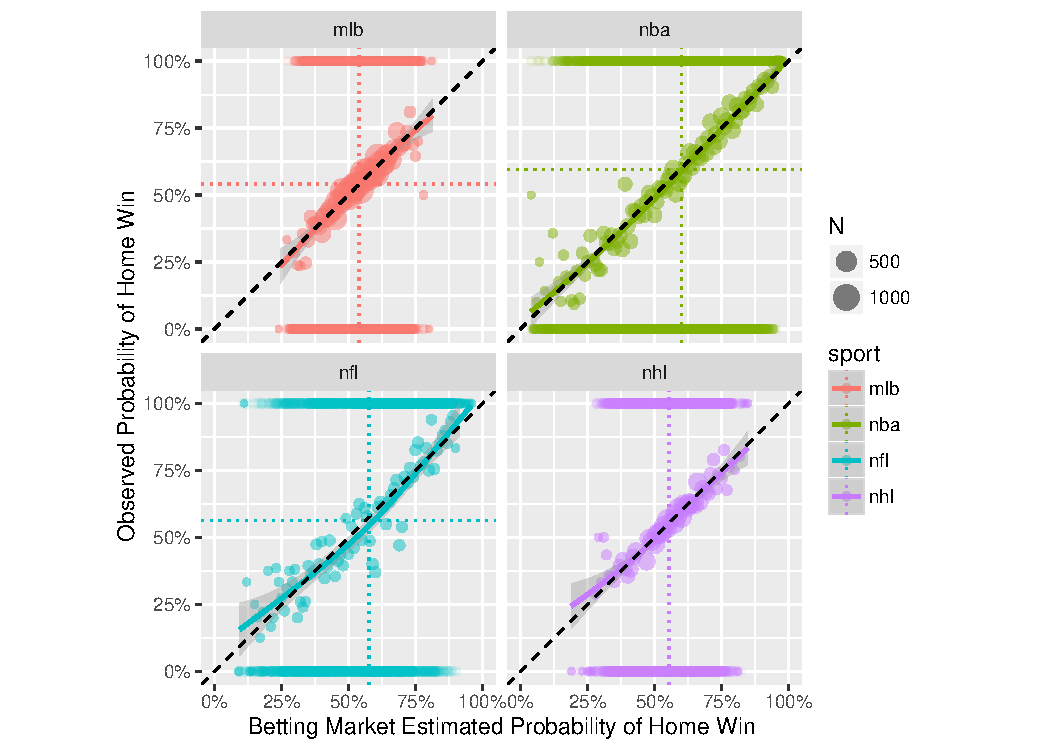
\includegraphics[width=\maxwidth]{figure/betting-1} \caption[Accuracy of probabilities implied by betting markets]{Accuracy of probabilities implied by betting markets. }\label{fig:betting}
\end{figure}


\end{knitrout}
\end{frame}

\section{Model}
\begin{frame}
For sport $q$, in season $s$, in week $k$: 
$$
logit(p_{(q,s,k)}) \sim N(\mathbf{\theta_{(q,s,k)}}\mathbf{X}_{q,s,k} + \alpha_{q_0}\mathbf{J}_{g_{q,s,k}} + \mathbf{\alpha}_{q}\mathbf{Z}_{q,s,k}, \tau^{2}_{q,game}\mathbf{I}_{g_{(q,s,k)}}) \,, 
$$

$$
\theta_{(q,s+1,1)} | \gamma_{q,seas}, \mathbf{\theta_{q,s,g_{q,s,.}}}, \tau^{2}_{q,seas},  \sim N (\gamma_{q,seas}\mathbf{\theta}_{(q,s,g_{q,s,.})},(\tau^{2}_{q,seas})I_{t_{q}})
$$
and 
$$
\theta_{(q,s,k+1)} | \gamma_{q,week}, \mathbf{\theta_{q,s,k}}, \tau^{2}_{q,week},  \sim N (\gamma_{q,week}\mathbf{\theta}_{(q,s,k)},(\tau^{2}_{q,week})I_{t_{q}})
$$
\end{frame}

\begin{frame}{Priors}
For sport $q$, for week $k=1$ and season $s=1$:\\
Team Strength:\\
$$
\theta_{(q,1,1)i} \sim N(0, \tau^{2}_{q,season}) \,, \qquad \text{for } i \in 1, \ldots, t_{q}.
$$
Home Field Advantage:\\
$$
\alpha_{(q)j}\sim N(0, \tau^{2}_{q,\alpha}) \,, \qquad \text{for } j \in 1, \ldots, t^{\star}_{q}.
$$

Finally, we assume the following prior distributions: 

\begin{align*}
\tau^{2}_{q,game} &\sim \Gamma(0.0001,0.0001) &\qquad
  \alpha_{q} &\sim N(0,10000) \\
\tau^{2}_{q,season} &\sim \Gamma(0.0001,0.0001) &\qquad
  \gamma_{q,season} &\sim Uniform(0,2) \\
\tau^{2}_{q,week} &\sim \Gamma(0.0001,0.0001) &\qquad
  \gamma_{q,week} &\sim Uniform(0,2) \\
\tau^{2}_{q,\alpha} &\sim \Gamma(0.0001,0.0001) && \\
\end{align*}

\end{frame}


\section{Results}
\begin{frame}[fragile]
\begin{knitrout}
\definecolor{shadecolor}{rgb}{0.969, 0.969, 0.969}\color{fgcolor}
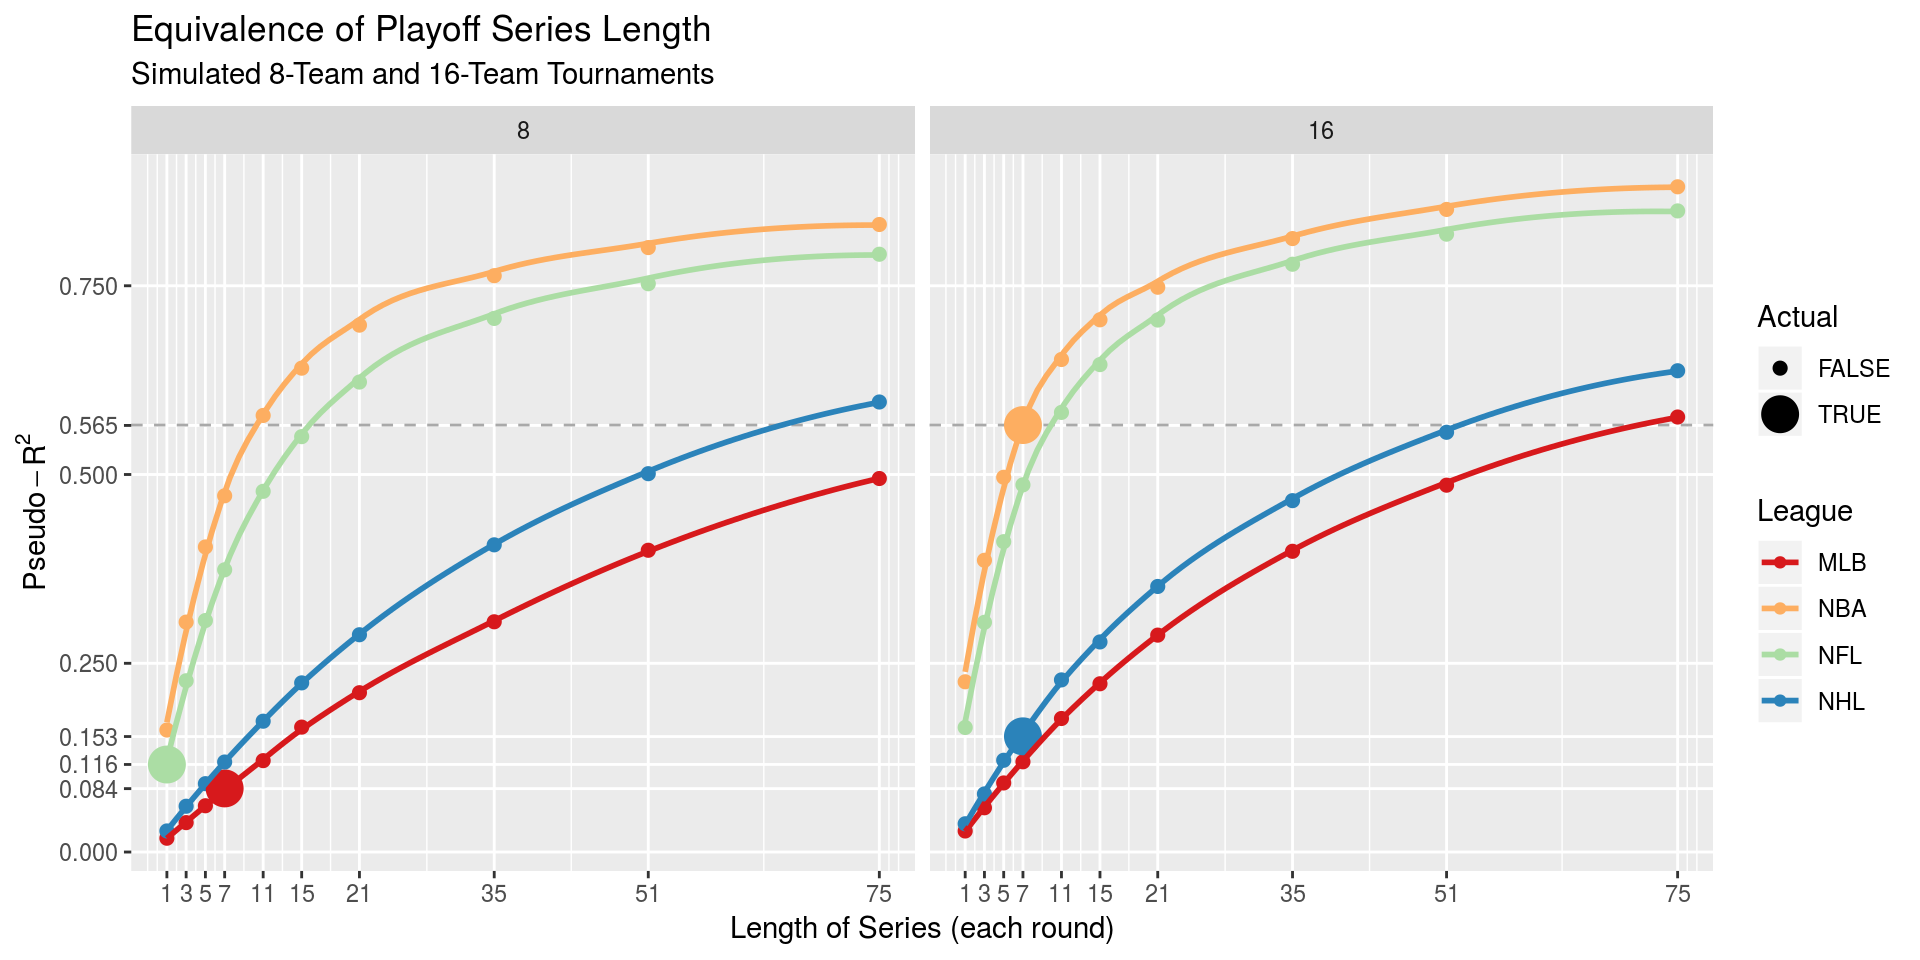
\includegraphics[width=\maxwidth]{figure/unnamed-chunk-2-1} 

\end{knitrout}
\end{frame}

\begin{frame}[fragile]
% latex table generated in R 3.3.1 by xtable 1.8-2 package
% Fri Oct 14 18:41:46 2016
\begin{table}[ht]
\centering
\begin{tabular}{lrrrrrr}
  \hline
sport & N & $\alpha$ & $\gamma_s$ & $\gamma_w$ & $\sigma_s$ & $\sigma_w$ \\ 
  \hline
mlb & 4000 & 0.160 & 0.619 & 1.002 & 0.009 & 0.001 \\ 
  nba & 4000 & 0.502 & 0.617 & 0.977 & 0.196 & 0.028 \\ 
  nfl & 4000 & 0.358 & 0.688 & 0.978 & 0.108 & 0.021 \\ 
  nhl & 4000 & 0.222 & 0.543 & 0.993 & 0.015 & 0.003 \\ 
   \hline
\end{tabular}
\caption{Summary of means from posterior draws for parameters.} 
\label{tab:params}
\end{table}

\begin{itemize}
\item $\alpha$: Home advantage
\item $\gamma_w$ and $\gamma_s$ autoregressive terms for week and season, respectively.
\item $\sigma_w$ and $\sigma_s$ variance terms form the $\theta$'s for week and season, respectively.  
\end{itemize}
\end{frame}

\begin{frame}[fragile]
\begin{knitrout}
\definecolor{shadecolor}{rgb}{0.969, 0.969, 0.969}\color{fgcolor}
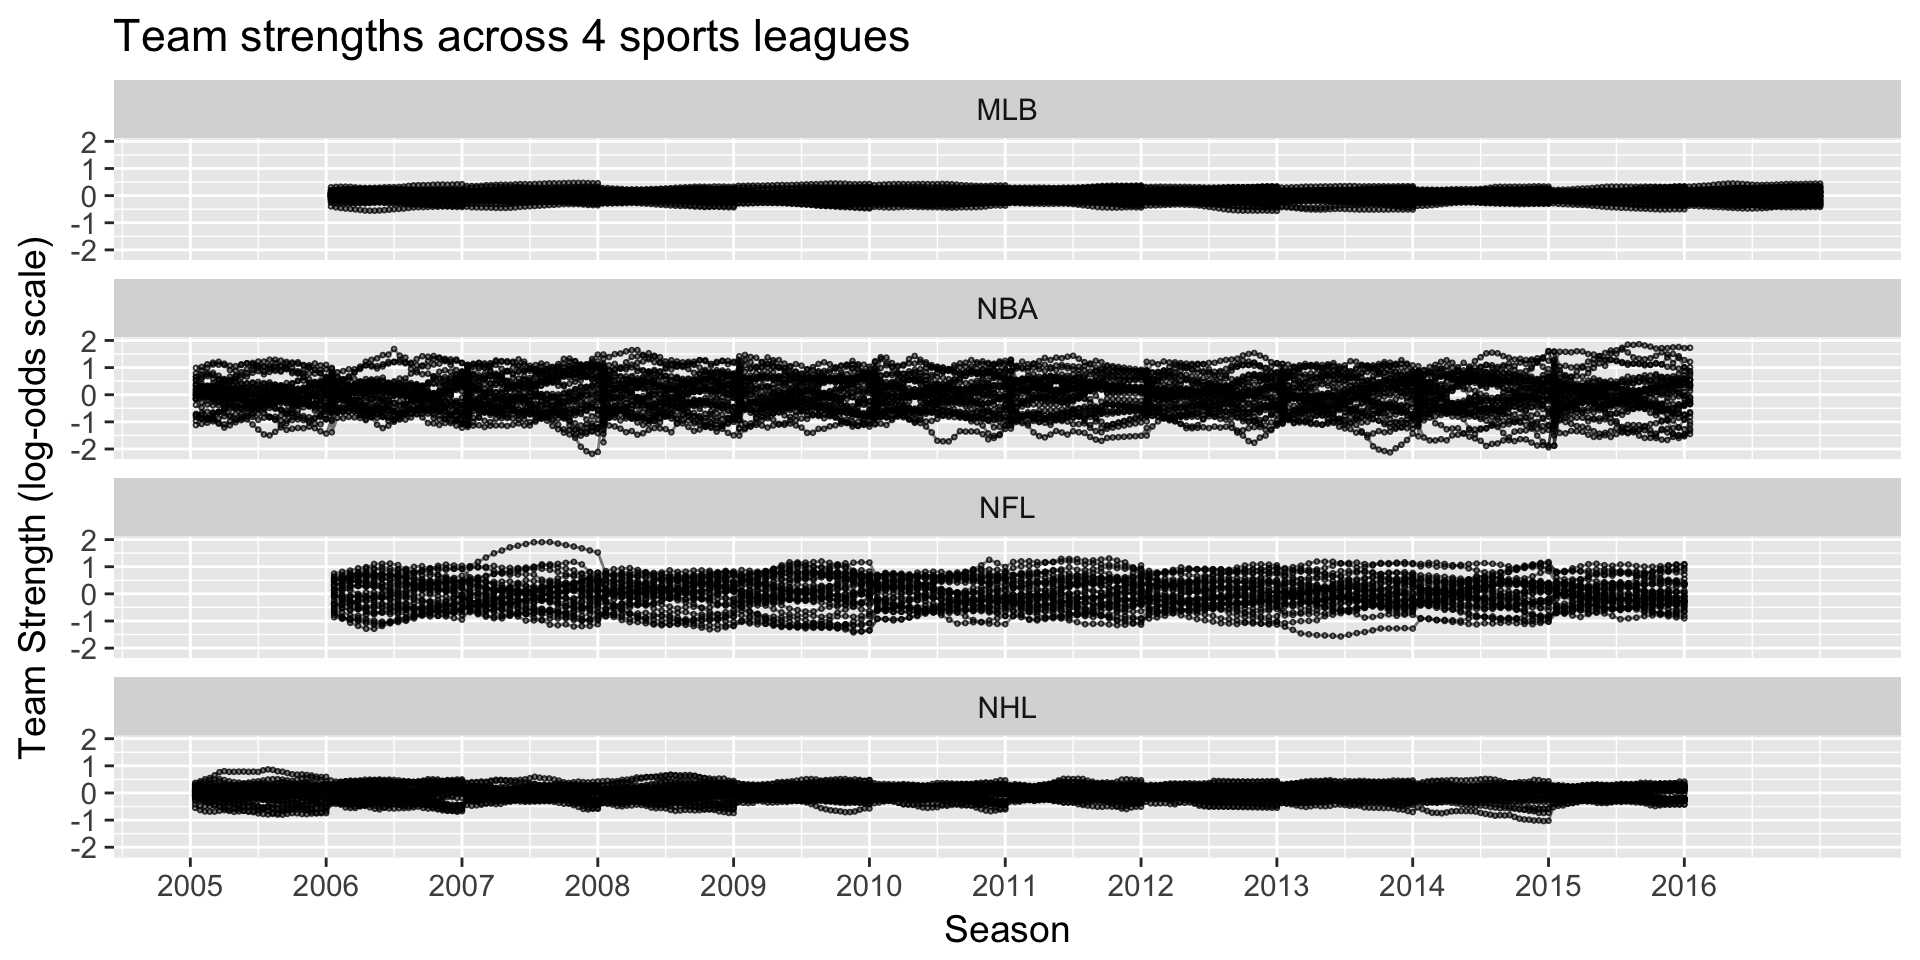
\includegraphics[width=\maxwidth]{figure/unnamed-chunk-4-1} 

\end{knitrout}
\end{frame}

\begin{frame}[fragile]
\begin{knitrout}
\definecolor{shadecolor}{rgb}{0.969, 0.969, 0.969}\color{fgcolor}
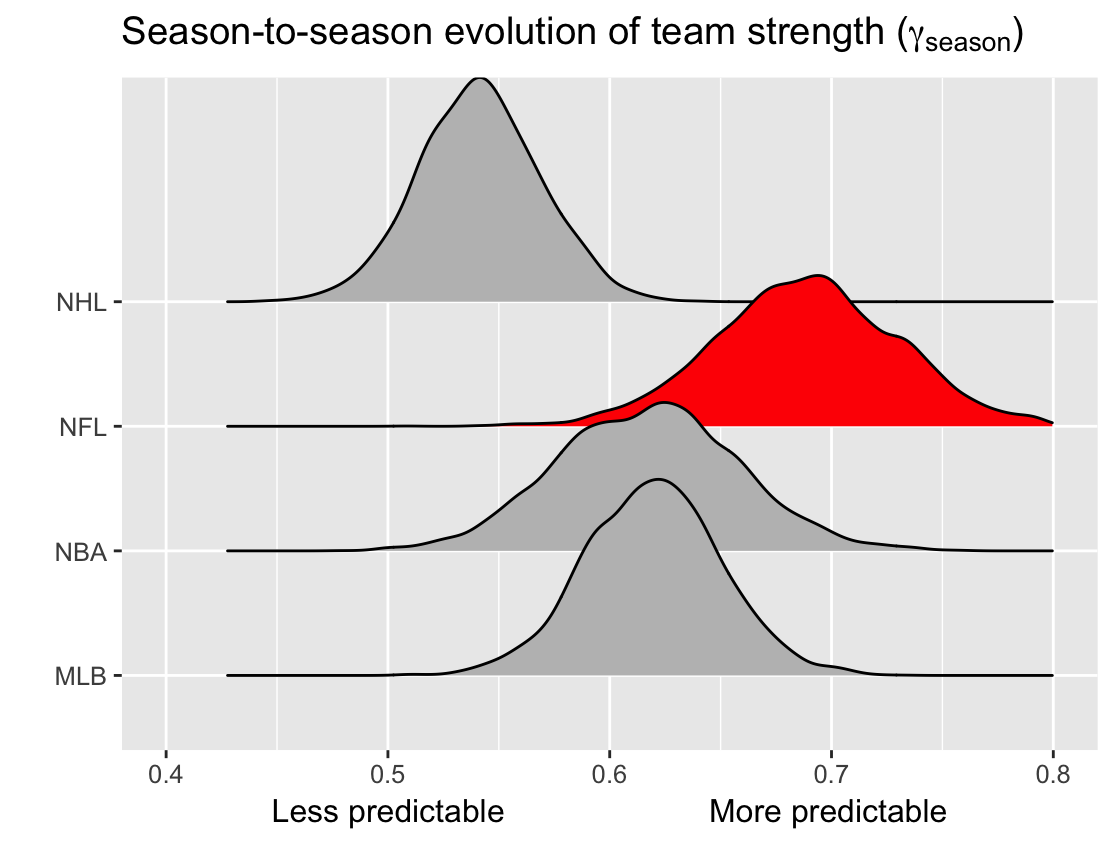
\includegraphics[width=\maxwidth]{figure/unnamed-chunk-5-1} 

\end{knitrout}
\end{frame}

\begin{frame}[fragile]
\begin{knitrout}
\definecolor{shadecolor}{rgb}{0.969, 0.969, 0.969}\color{fgcolor}
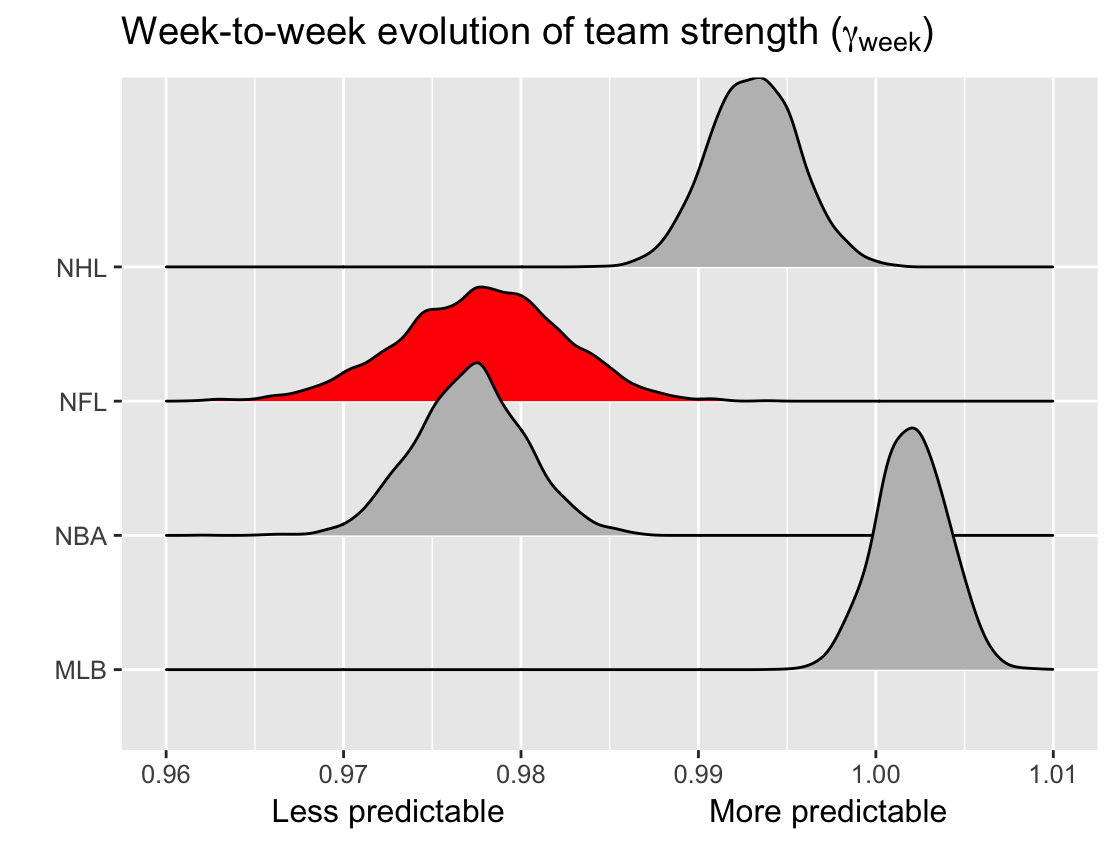
\includegraphics[width=\maxwidth]{figure/unnamed-chunk-6-1} 

\end{knitrout}
\end{frame}

\begin{frame}[fragile]
\begin{knitrout}
\definecolor{shadecolor}{rgb}{0.969, 0.969, 0.969}\color{fgcolor}
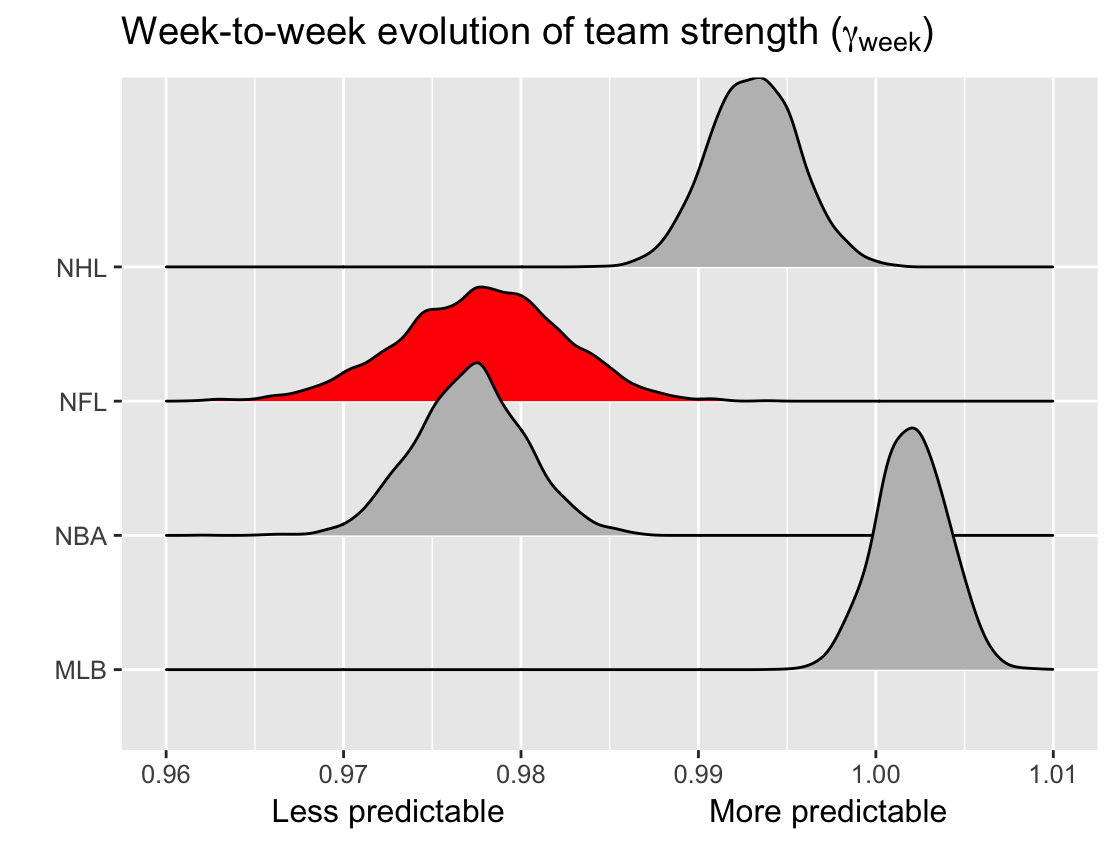
\includegraphics[width=\maxwidth]{figure/unnamed-chunk-7-1} 

\end{knitrout}
\end{frame}

\begin{frame}[fragile]
\begin{knitrout}
\definecolor{shadecolor}{rgb}{0.969, 0.969, 0.969}\color{fgcolor}\begin{figure}
\includegraphics[width=\maxwidth]{figure/sevenSeries-1} \caption[Probability top ranked team wins a postseason series by sport and opponent rank]{Probability top ranked team wins a postseason series by sport and opponent rank}\label{fig:sevenSeries}
\end{figure}


\end{knitrout}

\end{frame}

\subsection{Post-season}
\begin{frame}{Post-season}
\begin{itemize}
\item Best team wins most often in the NBA.  Number 1 beats 2 about 60\% and 1 beats 8 80\%. 
\item Better NFL team wins between 60-70\%. 
\item In the NHL and MLB, better teams wins between 55-65\%. 
\end{itemize}
\end{frame}


\begin{frame}{How many games? }
need to be played so we match the certainity of the NBA?  
To ensure 80\% (NBA level) chance the better team beats the 8th best teams we would need: 
\begin{itemize}
\item NFL: Best of 9
\item NHL: Best of 39
\item MLB: Best of 51
\end{itemize}

To ensure 72\%  (NBA level) chance the better team beats the 4th best teams we would need: 
\begin{itemize}
\item NFL: Best of 9
\item NHL: Best of 41
\item MLB: Best of 55
\end{itemize}
\end{frame}


\section{Conclusions}
\begin{frame}
\begin{itemize}
\item As a given time point, NBA and NFL have a much wider variety of team strengths than the MLB and NHL.  
\item Teams in the NBA (largest reversion), NFL, NHL tend to revert to the league-wide mean in the long run from week to week. .
\item Team strengths in the MLB are essential a random walk from week to week.  
\item From season to season, NHL teams exhibit the largest reversion to the league average (nearly 50\%).
\item The other three leagues are between 25\% and 40\%.  
\end{itemize}
\end{frame}

\begin{frame}
\begin{itemize}
\item The NBA home advantage is the largest of all four sports with a 0.52 increase in the log-odds of a home win.  
\item Further, home advantage varies significantly between arenas in the NBA and NHL, but not NFL or MLB.  
\item An NBA team with a typical home advantage can expect to win 62.7\% of home games against a like-caliber opponent; for Brooklyn, the corresponding figure is 60.3\%, while for Denver, 68.6\%.
\end{itemize}
\end{frame}



\section{Future Work}
\begin{frame}{Future Work}
\begin{itemize}
\item Examine the impact of imbalanced schedules
\item Increase granularity (i.e. measure team strength daily rather than weekly)
\item Study tanking
\item Expand the model beyond an auto-regressive structure (e.g. Stochastic Volatility Process)
\end{itemize}
\end{frame}




\end{document}




